%%%%%%%%%%%%%%%%%%%%%%% file template.tex %%%%%%%%%%%%%%%%%%%%%%%%%
%
% This is a template file for the LaTeX package SVJour2 for the
% Springer journal "Machine Vision and Applications".
%
%                                    Springer Heidelberg 2004/11/04
%
% Copy it to a new file with a new name and use it as the basis
% for your article. Delete % as needed.
%
%%%%%%%%%%%%%%%%%%%%%%%%%%%%%%%%%%%%%%%%%%%%%%%%%%%%%%%%%%%%%%%%%%%

%
\documentclass[twocolumn,fleqn,runningheads]{template_files/svjour2}
%
\smartqed  % flush right qed marks, e.g. at end of proof
%
\usepackage{graphicx}
\usepackage{template_files/biograph}        % to allow for author biography at the end
\usepackage{booktabs}
\usepackage{tabu} % for full-width table
\usepackage{hyperref} % for links to references

\journalname{Internet of Things}
%
\begin{document}

\title{A Blockchain-based payment and management architecture for vending machines}
%\subtitle{An overview}

\author{Cem Basoglu\textsuperscript{1}, Kevin Schima\textsuperscript{2}}

\institute{Cem Basoglu \at
           Univ. of Appl. Sci., Minden, Germany \\
		   \email{cem.basoglu@fh-bielefeld.de} \and
		   Kevin Schima \at
           Univ. of Appl. Sci., Minden, Germany \\
		   \email{kevin.schima@fh-bielefeld.de}
}

\date{Submitted: 7/20/2018}
% The correct dates will be entered by the editor

\maketitle

\begin{abstract}
In context of rising pay-per-use business models, we envision a triangular profit-sharing business relationship between a vending machine manufacturer, contractors responsible for machine maintenance and location providers for machine installation. Besides, we facilitate the future adoption of this architecture by developing a system which also provides benefits for vending machine customers. We identify the lack of trust as the main problem in a centralized profit-sharing system. 
Centralized systems do not provide a trusted environment for all participants where manipulation of sales figures is impossible. 
In this paper, we propose an blockchain-based architecture for management and payment processing of this presented system. We compare the properties of different Distributed Ledger Technologies to implement a proof-of-concept by using a coffee machine.
\keywords{Distributed Ledger \and Blockchain \and Internet of Things \and Smart Contracts \and Vending machines}
\end{abstract}

\section{Introduction}
According to the Gartner Hype Cycle for emerging technologies, blockchain has just passed the peak of inflated expectations \cite{TopTrend28:online}. While the technology itself enables the creation of decentralized applications with immutable and tamper proof transactions, without the need of a controlling third party, it is currently primarily used in FinTech solutions or namely in cryptographic currencies. The peak of the hype cycle is associated with more than 1,600 different cryptocurrencies with a market capitalization of around 350 billion dollars \cite{AllCrypt83:online}, and in contrast only a relatively small number of proof of concepts for other applications \cite{8338177,8016254,8306880,DBLP:journals/corr/abs-1804-00658,PlaTIBART}. To overcome the phase of disillusionment and reach the plateau of productivity, useful mainstream and enterprise applications are required. This can be accomplished by transforming existing applications to create more efficient, secure and cost-effective solutions based on blockchain technologies \cite{REYNA2018173}. At the same time, the blockchain technology creates opportunities for new applications that were previously difficult or impossible to implement, such as tracking goods in a supply chain \cite{doi:10.1002/isaf.1424} or machine-to-machine payments \cite{8016254}.

In this context, the scope of this paper is to examine various blockchain platforms and technologies for the capability of processing mobile micro-payments, inventory management and settlements in vending machines. Based on these findings we propose a novel solution and implement a proof of concept by using suitable blockchain platform and a coffee machine to represent the vending machine. The design goal of the proposed solution is the exclusive use of blockchain technologies without the need for additional cloud-based services.
\section{Background\textsuperscript{2}}
\bgroup
\def\arraystretch{2}% 
\begin{table*}[t]
\caption{Comparison of distributed ledger technologies (July 2018), extended from \cite{pustivsek2018approaches}}
\begin{tabu} to \textwidth {lXXXX}
   \toprule
 & Bitcoin & Ethereum & Hyperledger Fabric & IOTA \\ \midrule
 Native cryptocurrency & Yes & Yes & No & Yes \\
 Decentralized applications & No & Yes & Yes & No \\
 Transaction fee & Yes & Yes & No & No\\
Transaction fee/speed & \$0.15 / 10 min.\cite{bitcoinfees:online} & \$0.28 / 2 min.\cite{ethgasstation:online} & Instant & 5 min\cite{tanglemonitor:online}\\ 
 Transactions per sec. & 3-7 & 7-15 & 3500 \cite{androulaki2018hyperledger} & 10 \\ 
 Network type & Public & Public / Private  & Private & Public \\ 
 Network access & Permissionless & Permissionless & Permissioned & Both \\ 
 Anonymous accounts & Yes & Yes & No & Both \\ 
 State channels & Lightning & \mu Raiden, Raiden & Not required & Flash channels \\ 
 Suitable for IoT & No & With constraints  & Yes & Yes\\ 
 Suitable for DApps & No & Yes & Yes & No \\ \bottomrule
\end{tabu}
\raggedright {}
\label{table:dl_comparison}
\end{table*}
\egroup
Blockchain platforms in general provide a distributed data structure, the blockchain and a consensus mechanism, which allows to find a mutual agreement about the state of the blockchain. The blockchain data structure consists of blocks, were all transactions are stored in, and additionally contain a hash of the previous block. (Fig. \ref{fig:blockchain})
The basis of these system is, that every participant involved, stores the entire blockchain history, a manipulation of the state would require to alter data on the majority of system peers.
\begin{figure}[h]
    \centering
    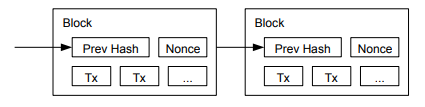
\includegraphics[width=0.5\textwidth]{assets/blockchain.png}
    \caption{Blockchain structure}
    \label{fig:blockchain}
\end{figure}
Blockchain is only one type of Distributed Ledger Technology (DLT), in a later section we will describe IOTA as another approach, which does not rely on the linear blockchain data structure.
The blockchain-based cryptocurrencies Bitcoin, Ethereum and Co. allow the settlement of financial transactions via a distributed, trusted ledger stored within the blockchain. 
But one of the most obstructive properties of these \\ blockchain-based systems, for Internet-of-Things (IoT) and micro-payment systems in general, is the occurrence of transaction fees and the required storage capacity to persist the distributed ledger.
IoT devices equipped with temperature and humidity sensors for example, continuously transmit a stream of small data packages. Thus, the usage of popular public block-chain systems e.g. Bitcoin or Ethereum, which incorporate transaction fees as a means for preventing transaction spam, is not economically viable. For use cases that are not built around a high distrust of every participant involved, permissioned blockchain solutions seem to be a promising approach, because consensus of transaction history is reached by a limited amount of peers. The blockchain data structure is the most popular Distributed Ledgers Technology (DLT). Recently an entire different architecture in form of the cryptocurrency IOTA emerged, which has been developed for IoT device use cases. It does not incorporate transaction fees and does not suffer from typical blockchain scalability problems. In Table \ref{table:dl_comparison} we compare the properties of different distributed ledger technologies side-by-side, additionally we provide a deeper explanation of these technologies in the following sections. 

\subsection{Bitcoin}
Bitcoin, proposed 2007 by the pseudonym Satoshi Nakamoto, was the first cryptocurrency, which solved the double spending problem by a distributed network consensus mechanism. In its initial design, Bitcoin has a very limited smart contract capability. Smart contract code needs to be executed by every node for verification, which entails the risk that a given code might be too computational expensive and slow down or even halt the network. While Ethereum, as described in the following section, counters this problem with defined costs for every computational operation performed, Bitcoin was not designed with these capabilities at its inception.
\\ \\
As other blockchain platforms, Bitcoin also suffers from a transaction bottleneck, mainly caused by a system design that enforces the generation of a new block roughly every 10 minutes and the fixed maximum block size of 1 Megabyte, which limits the number of transactions a block can hold. This bottleneck, resulted in peaks with high numbers of unprocessed transactions and fees of over 50 Dollar in December 2017 \cite{bitcoin-txfee:online} for a single transaction.
To circumvent these limitations, numerous blockchain forks emerged, which either increase the block size limit, reduce the block time, or both.\\ \\
While numerous proposals exist to extend Bitcoins capabilities regarding transaction throughput or scalability in general, these proposals are still not in widespread use or not yet completed.\cite{poon2016bitcoin}

\subsection{Ethereum}
Ethereum was developed upon the core principles of the Bitcoin protocol, while extending it in various ways that were not foreseeable at the introduction of Bitcoin and optimizing it for mass adoption. One of the shortcomings of Bitcoin, was the lack of a Turing-complete programming language to allow smart contracts. Smart Contracts
enable a the transparent implementation of business logic on a blockchain for all participants who want to interact with it.
Ethereum implemented the Ethereum Virtual Machine (EVM) which handles internal state, computation and allows smart contracts to be deployed to the blockchain. Transactions can not only be send to other users but also to smart contracts, where they invoke contract functions, which in turn could invoke other smart contracts themself.
\\
The extensive smart contract capabilities resulted in the tokenization of various assets and the ability to trade them on the Ethereum network. \\ \\
With the ERC-20 token standard, which provides common rules for token transfers, interaction and made it easy to implement and issue tokens, a multitude of token smart contracts emerged. Today, about 99,000 known ERC token contracts exist on the Ethereum blockchain \cite{Etherscan1:online}, many of them providing services based on these tokens. The widespread adoption of ERC tokens and related services has led to the largest community and development ecosystem for smart contracts to date.
\\
To solve different scalability problems, numerous side projects are under development to provide off-chain solutions \cite{eberhardt2017or} or extend Ethereums capabilities, similar to Bitcoin.

\subsection{IOTA}
IOTA is a cryptocurrency introduced in 2016 \cite{popovtangle:online}, which does not use a typical blockchain data structure. It uses a data structure, called \textit{Tangle}.
\begin{figure}[ht]
\centering
  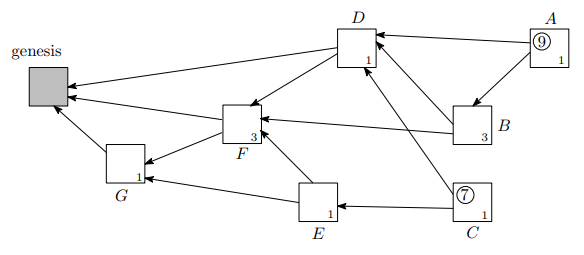
\includegraphics[width=0.5\textwidth]{assets/tangle.png}
\caption{Tangle data structure}
\label{fig:tangle}
\end{figure}
As depicted in Figure \ref{fig:tangle}, every transaction validates two former transactions. In this system, more activity in the IOTA network leads to faster validation and confirmation of transactions and theoretically unlimited scalability.
\\
While the  blockchain architecture of Bitcoin and Ethereum with their finite block size and enforced block time, limits the number of transaction in a certain time frame, IOTA does not have these constraints. But the advantages of IOTAs architecture only become apparent when a certain size of the network is reached. It is designed as a protocol for the rapidly rising number of IoT devices, for a machine-to-machine (M2M) economy, where devices interact with each other autonomously. In this regard, IOTA would be an enabler for the processing of a tremendous amount of transactions. Currently, the IOTA network handles about 10 transactions per second while after a stress test at the end of the year 2017 the IOTA team reported 100 transactions per second. As mentioned earlier, theoretically IOTA is able to outperform blockchain based technologies, if the network size i.e. the transaction throughput, reaches a certain threshold. \\

The IOTA Foundation itself describes various future use cases for IOTA: Over-the-air updates for IoT devices, data marketplaces, supply-chain management and more.
IOTA is an interesting approach, with its clear focus on IoT devices and enabling a machine-to-machine economy, in this early stage of the IOTA network, however, it is not an ideal solution for instant payments.\\

\subsection{Hyperledger Fabric}
Hyperledger Fabric is a permissioned blockchain framework initially developed by IBM and now part of the Linux Foundation. As a framework, it is not a single blockchain, but a basis to develop blockchain solutions for enterprise ecosystems \cite{androulaki2018hyperledger}. Contrary, to the other proposed solutions, it does not include a native cryptocurrency. Its Byzantine-fault tolerant (BFT) consensus mechanism \cite{castro1999practical} is designed for an environment where all participants are explicitly identified and have a common goal in general, which does not imply that all parties trust each other fully. Besides, the default consensus mechanism is replaceable, to allow different approaches depending on use case. For smart contracts, Fabric allows the usage of standardized programming languages (Go, NodeJS, Java) and does not integrate its own language, hence the project describes itself as "the first distributed operating system for permissioned blockchains" \cite{androulaki2018hyperledger}.
\\
Fabrics \textit{membership service provider} (MSP) is responsible for authentication of all network participants, it issues cryptographic certificates for interaction with the network and checks their validity. The network can be governed by multiple MSPs, in many Fabric implementations this is a committee representing all stakeholders.
\\ \\
On the Fabric platform, every smart contract (in Fabric terms: chaincode) runs in its own docker container, separated from other chaincodes or the host system. Additionally, by design, the host system is agnostic of the chaincodes underlying programming language.
\\ \\
Fabric also integrates the concept of (transaction) channels, which allows fine-grained control about which transaction information is visible to participants. With this, confidential transactions can take place on the Fabric blockchain, while complying with f.g. legal restrictions.
By design, the chaincode is not inevitably executed by every peer of the system, this is a matter of individual configuration (endorsement policy), which can significantly increase the overall transaction throughput of the system, compared to Bitcoin or Ethereum, where execution is required by every peer.
\section{Related work\textsuperscript{2}}
Gao et al. \cite{8338177} proposed a platform to let electric vehicles (EVs) participate in Vehicle-to-Grid (V2G) networks for bidirectional electric energy transmission and payment settlement for consumed energy. They argued that their proposed system would allow valuable statistical information for load forecasting, price prediction or optimal energy consumption scheduling. Their concept was implemented with Hyperledger Fabric and they also observed the significantly increased transaction throughput, a permissioned blockchain approach can provide, compared to public blockchains such as Bitcoin or \\ Ethereum.

Lundqvist et al. \cite{8016254} realized a \textit{smart cable}, which pays the \textit{smart socket} counterpart for electricity consumption via Bitcoin. They also identified transaction fees as the main problem for micro-payment use cases, which they mitigated by batching of transactions. They concluded that this approach implies, that with increasing transaction batch-size for reducing relative proportion of fees, the risk for fraud equally increases.  

Novo \cite{8306880} proposed a concept based on a private \\ Ethereum blockchain for communication and access management of IoT devices. Each device communicates with the so called \textit{management hub} and  does not interact directly with the blockchain. They conclude that with the rapidly rising number of IoT devices connected to the internet, centralized management systems would not be able to handle the transaction quantity and minimize reliability by forming a single point of failure. They also observed, that computational constrained IoT devices would need an intermediary layer to connect to blockchain platforms because of storage space limitations.

Strugar et al. \cite{DBLP:journals/corr/abs-1804-00658} followed a machine-to-machine economy driven approach, by envisioning a charging architecture and billing system for Electric Autonomous Vehicles (EAVs) using the IOTA cryptocurrency for payments, avoiding the occurrence of transaction fees. They emphasized on the early stage of IOTA development and existing security concerns, regarding the cryptographic implementations, not following best practices. Albeit, the approach was convincing, their work was theoretical without an proof-of-concept implementation.

With PlaTIBART, Walker et al. \cite{PlaTIBART} proposed a platform for development, deployment, execution, management and testing of IoT blockchain applications. They criticized the lack of a fault tolerant, secure Ethereum client with an emphasize to IoT devices and pointed out the necessity for such a platform through the large number of attacks and hacks on Ethereum smart contracts, where Ether worth millions of Dollars got stolen.

Unlike this paper, none of the introduced papers emphasized on a payment and management system where different parties have a profit-sharing business model as its common with pay-per-use systems.

\section{Method\textsuperscript{1}}
\begin{figure}[ht]
    \centering
    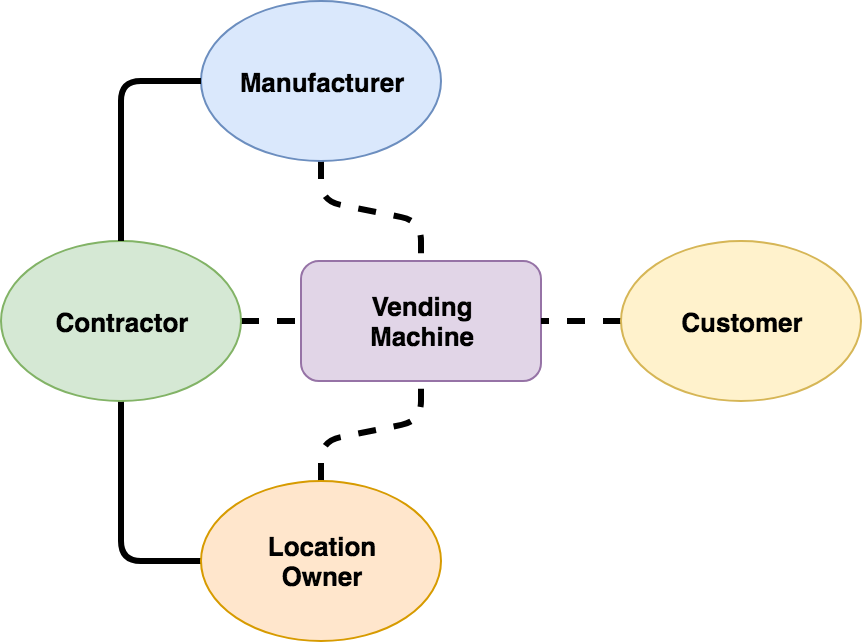
\includegraphics[width=0.4\textwidth]{assets/relations.png}
    \caption{Actors of the systems}
    \label{fig:relations}
\end{figure}
The typical business models for vending machines consists of multiple \textit{stakeholders} (see Figure \ref{fig:relations}), where at least a \textit{location owner} and a \textit{contractor} is involved. The contractor can operate independently or in a larger scale business model as shown in Figure \ref{fig:relations2}, in cooperation with the vending machine \textit{manufacturer}. The contractor is responsible for item refilling and maintenance of a vending machine whereby the location owner provides the physical space for a vending machine installation. Regardless of the business model scale, all actors share the profit, which requires a certain degree of mutual trust. For example, all stakeholders must trust the contractor's reports on the vending machine's revenues.
\begin{figure}[ht]
    \centering
    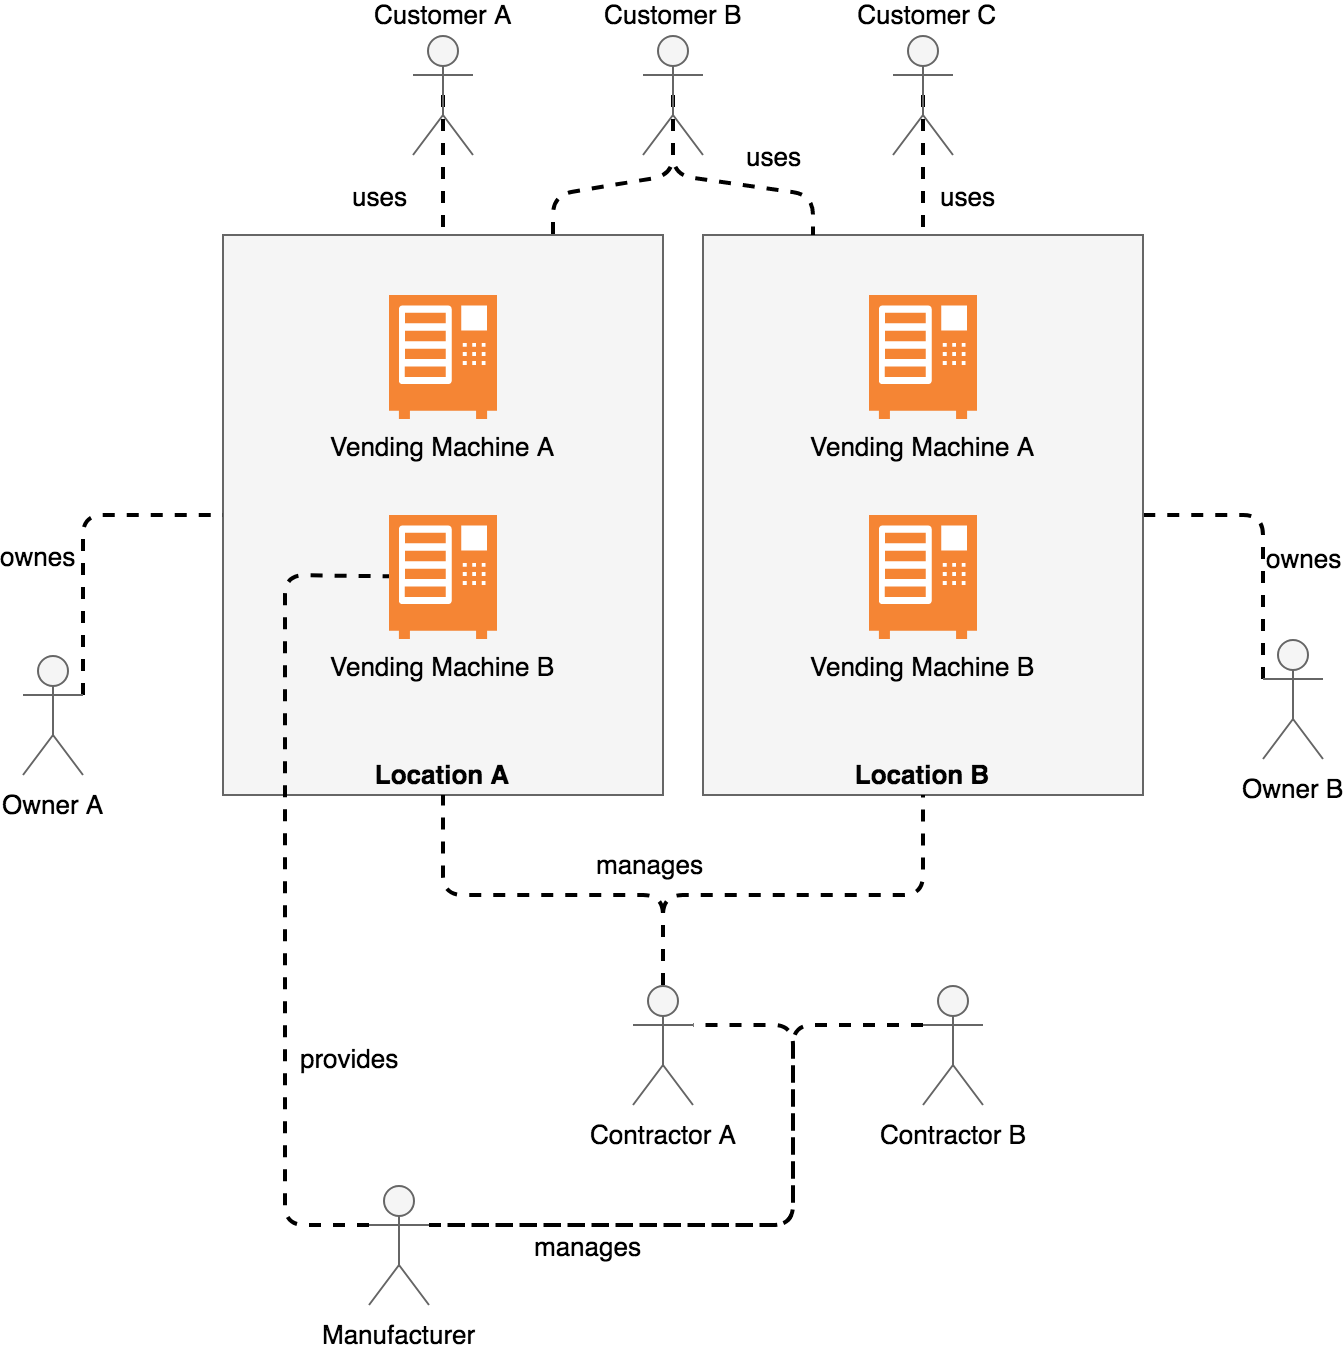
\includegraphics[width=0.49\textwidth]{assets/relations2.png}
    \caption{Relationships between the actors}
    \label{fig:relations2}
\end{figure}
A second view point is the \textit{customers} perspective, who prefers an effortless and quick electronic payment at the vending machine. The customer uses the vending machines on different locations but might be accustomed to use the same payment method on all locations. \\
For both view points, a blockchain technology can help to solve the described issues. Due to the distributed ledger technology, each stakeholder manages a copy of the ledger, which provides transparency in the system. At the same time, the blockchain technology forces all stakeholders to agree on the global state of the ledger to avoid manipulations of the ledger. These requirements can be summarized as the following. \\
\begin{itemize}
  \item quick, effortless payments for customers
  \item low payment processing time to avoiding queues in rush hours
  \item easy and intuitive use by customers
  \item comparable or better user experience for customers, compared to cash payment
  \item transparency for all actors
  \item no or low transactions fees for payment processing
  \item no costs for device management
  \item ability to integrate additional payment providers
\end{itemize}
The proposed system aims to implement a management architecture for pay-per-use business cases, especially for vending machines, with percentage-wise profit sharing, inventory management and payment processing, on a blockchain. A blockchain approach is being pursued to create a transparent, trusted environment for all stakeholders of the system, more precisely the manufacturer, the contractors and the location providers. From an user-experience oriented point of view, payment transaction speed should be comparable to familiar methods, like cash payment or EC payment, to incentivize acceptance and adoption. With most blockchain based solutions, this criterion is difficult to fulfill, while maintaining a secure transaction confirmation threshold. The nature of blockchain based solutions allows a high level of reliability and trust because of a redundant number of peers as an integral part of the consensus mechanism, which eliminates a single point of failure.

\subsection{Approach}

As described in the Background section, many blockchain technologies are already in active use and common cryptocurrencies like Bitcoin or Ethereum can rather easily be acquired through a myriad of specialized cryptocurrency exchanges. Though, the transaction confirmation time, easily taking a few minutes on most blockchain platforms, does not fulfill an essential requirement for our architecture. The unpredictable and highly fluctuating transaction fees, which we already recognized in the background section as a main obstacle, would hamper the adoption of the proposed system and render every advantage, the system provides for management of vending machines, insignificant. \\
Of all distributed ledger platforms discussed, only the Ethereum Platform and the Hyperledger Fabric Framework allow the implementation of business logic in smart contracts which is essential for transparency in this pursued triangular business model. But with Ethereum, not only the payment process itself would result in transaction fees, also every management operation that invokes the smart contract, for example updating prices of items, creates costs. As of this, the Hyperledger Fabric framework, with nearly instant transactions and no transaction fees, would be an ideal solution for implementation of the introduced architecture, but it lacks a native integrated cryptocurrency for monetary balance settlement, because of an enterprise oriented focus.

To develop a convincing solution, the proposed method uses a combination of both approaches, to achieve instant transactions and the usage of popular cryptocurrencies. For this, the business logic of the model described earlier in this chapter is implemented with the Hyperledger Fabric framework, which allows transparency and trust for all stakeholders involved. The business logic further maintains a balance for each customer, which can be redeemed on vending machines and recharged using popular cryptocurrencies. The customer is able to buy a product instantly at a vending machine and can make deposits to his account balance with various different payment providers, due to a modular approach. \\
Permissioned blockchains like Hyperledger Fabric require the authentication of each participant in the network. Therefore each stakeholder (see Figure \ref{fig:relations2}) and application component of the network (see Figure \ref{fig:systemarch}), uses x509 certificates for authentication. The certificate consist of a public and a private key and is used to sign every transaction, resulting from the interaction with the network, with the private key portion.

For the identification of the customer, we compared QR codes, NFC and Bluetooth technologies. Using a smartphone, the customer would be able to generate a unique QR code linked to his account and use it for identification at the vending machine. This approach would require a QR code reader for the recognition and a method to indicate a proper alignment between QR code reader and smartphone. We concluded that this concept is not ideal user-experience wise because of high probability of errors in the scanning process. \\
Perfectly suited to our use case, the range of Near Field Communication (NFC) is limited to close proximity between the user device and the NFC unit at the vending machine. Depending on the device manufacturer, smartphones support different standards and formats regarding NFC protocols. Apples iOS for instance, currently only supports tags in NFC Data Exchange Format \\ (NDEF) \cite{apple-nfc:online} and the API is not able to emulate NFC tags or more precisely, only supports reading of tags. The emulation of NFC tags is an essential aspect for identification of the user. In addition to the protocol restrictions of the iOS stack, the availability of NFC modules in smartphones further restricts this approach.\\
Because Bluetooth is supported in nearly all smartphones, we also evaluated an approach based on this technology. Apple iOS and Google Android both support the beacon Bluetooth profile, however the identification of individual users in a waiting queue might be problematic.

\subsection{System architecture and components}
\begin{figure}[ht]
\centering
  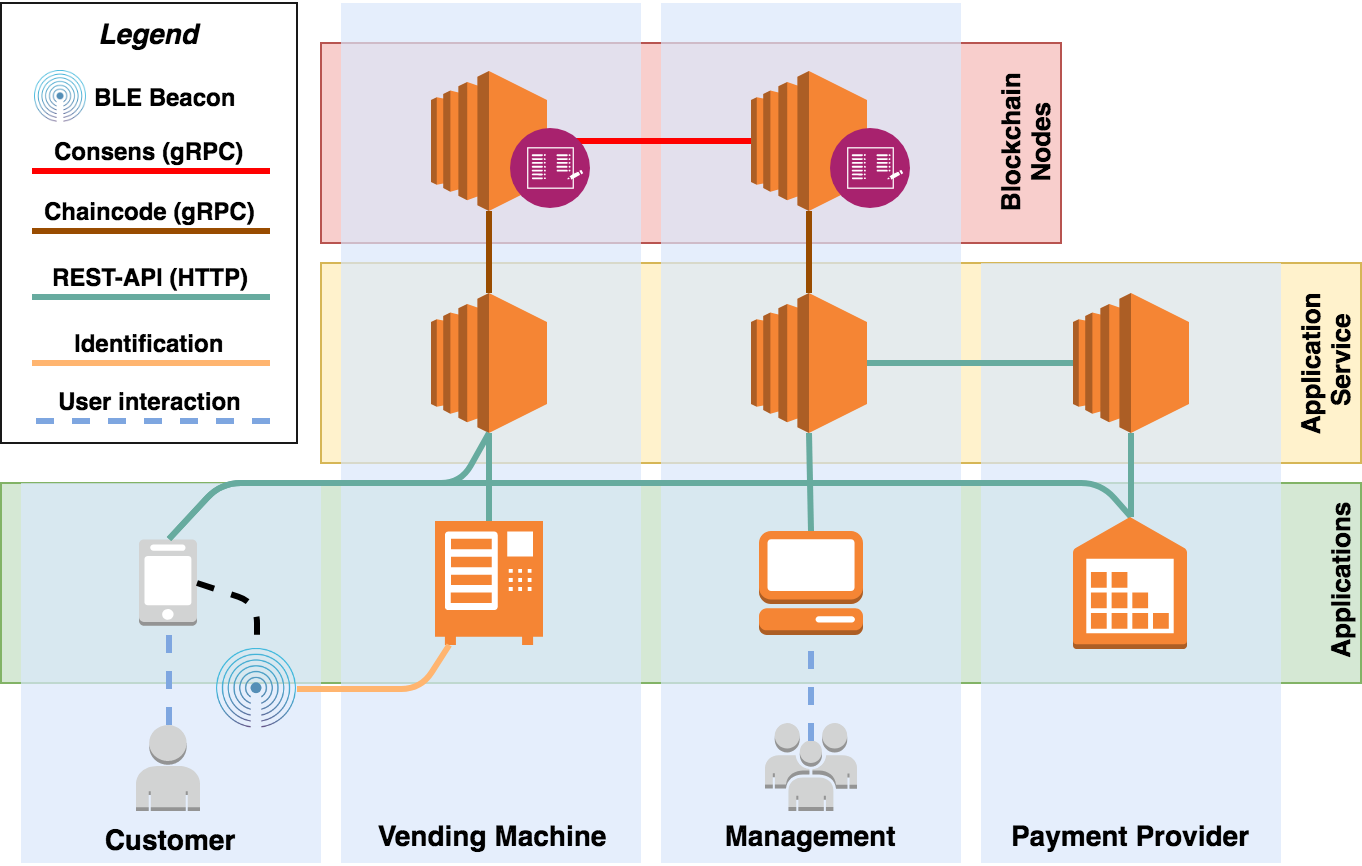
\includegraphics[width=0.5\textwidth]{assets/systemarch.png}
\caption{Architecture of the system components}
\label{fig:systemarch}
\end{figure}
Our proposed architecture is built on a layered structure of the components depicted in Figure \ref{fig:systemarch}, allowing a distributed deployment and a future functionality extension of the system through a loosely coupled design. \\
Because of the low availability of Near Field Communication (NFC) modules in smartphones and the intentionally restricted access to the lower layer of the NFC protocol in Apple devices, the proposed approach uses the Bluetooth beacon protocol for the identification of the customer at the vending machine. With the ongoing prevalence of NFC in smartphones and the programmatic access for third-party developers, user authentication at vending machines via NFC might get the preferred technique.\\
The system components are mainly developed using NodeJs and Typescript. The NodeJS ecosystem provides powerful tools and components for cross-platform projects, while allowing the reuse of common parts of the application between the different platforms like a mobile application, a web application or even embedded devices. In the following sections, we provide a description of the layers and components in detail.

\subsubsection{Blockchain nodes}
Each vending machine operates a blockchain node or \textit{peer} in Hyperledger Fabric terms, in order to increase protection against manipulation. For vending machines with a lower computational power, it is also possible to group several vending machines, based on the location or other criteria and use an edge device or even a cloud based service to operate the peer. 

Optionally, each stakeholder can also operate a peer with the full copy of the distributed ledger. Because multiple peers share the state of the blockchain, where all payments transactions get stored, no stakeholder is able to manipulate or forge earnings, which satisfies the requirement for profit-sharing business models. 

The logic of the business model is implemented in the chaincode of the Fabric framework and ensures that no chaincode invocation violates these rules. For instance the chaincode ensures that a customer is not able to purchase a product which exceeds the credits available on his account.

\subsubsection{Application service}
The application service layer consists of a REST service for the mobile application, vending machine and the management application described the next sections. The service is secured by the x509 certificate described earlier in this chapter and provides access to the network of Hyperledger Fabric peers. 

Depending on the payment provider, the application service layer also includes a service for the payment method which is responsible for the approval of a transactions, received from an external system or blockchain. It acts as a gateway between the proposed system and the external payment provider and deposits the transactions to the account of the customer as soon as they are approved. This decouples the transaction approval time described in the Section Background, from the actual payment process at the vending machine.

\subsubsection{Vending machine}
The vending machine dispenses goods such as food or drinks when a payment is received. Like described in the introduction of the chapter, the proposed method uses the Bluetooth Beacon protocol for identification of the customer. In this process, the customer selects the wanted product and is then requested to place the Beacon advertised by the mobile application on the smartphone to a specific area of the vending machine. The vending machine reads the account linked with the advertised beacon from the distributed ledger and requests to redeem the amount of the selected product. If the invocation of the redeem function in the chaincode succeeds, the requested good is dispensed.

\subsubsection{Mobile application}
\begin{figure}[ht]
\centering
  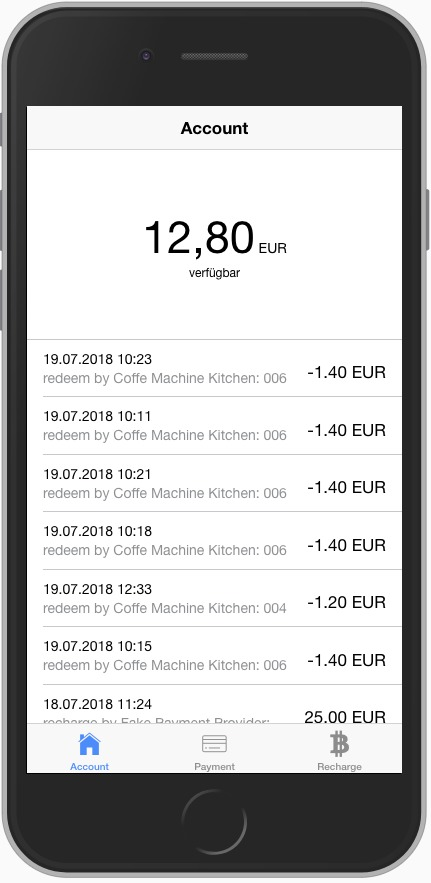
\includegraphics[width=0.45\textwidth]{assets/mobileapp.jpeg}
\caption{Account overview and transaction history}
\label{fig:mobile}
\end{figure}
Using the mobile application the customers is able to review the balance and the transaction history of his account (see Figure \ref{fig:mobile}). The transaction history includes the payouts from product purchases and deposits from payment providers. This provides the customer a transparent and verifiable insight into the account balance. 

For the identification, the customer must explicitly select the \textit{Payment} tab (see Figure \ref{fig:mobile}) in order to activate the advertisement of the Beacon. To minimize failures of accidentally advertised Beacons, the Beacon is disable when the another tab is selected or the application is closed. The advertised beacon contains the id of the account, which is then used by the vending machine to retrieve information about the customer.

To recharge credits to the customers account, the mobile application enables the customer to choose between different payment providers. Depending on the provider, the customer is redirected to the application of the provider or gets instructions to perform to complete the deposit. The payment provider service, described in the Section Application service, is triggered as soon the payment is completed.

\subsubsection{Management application}
\begin{figure}[ht]
\centering
  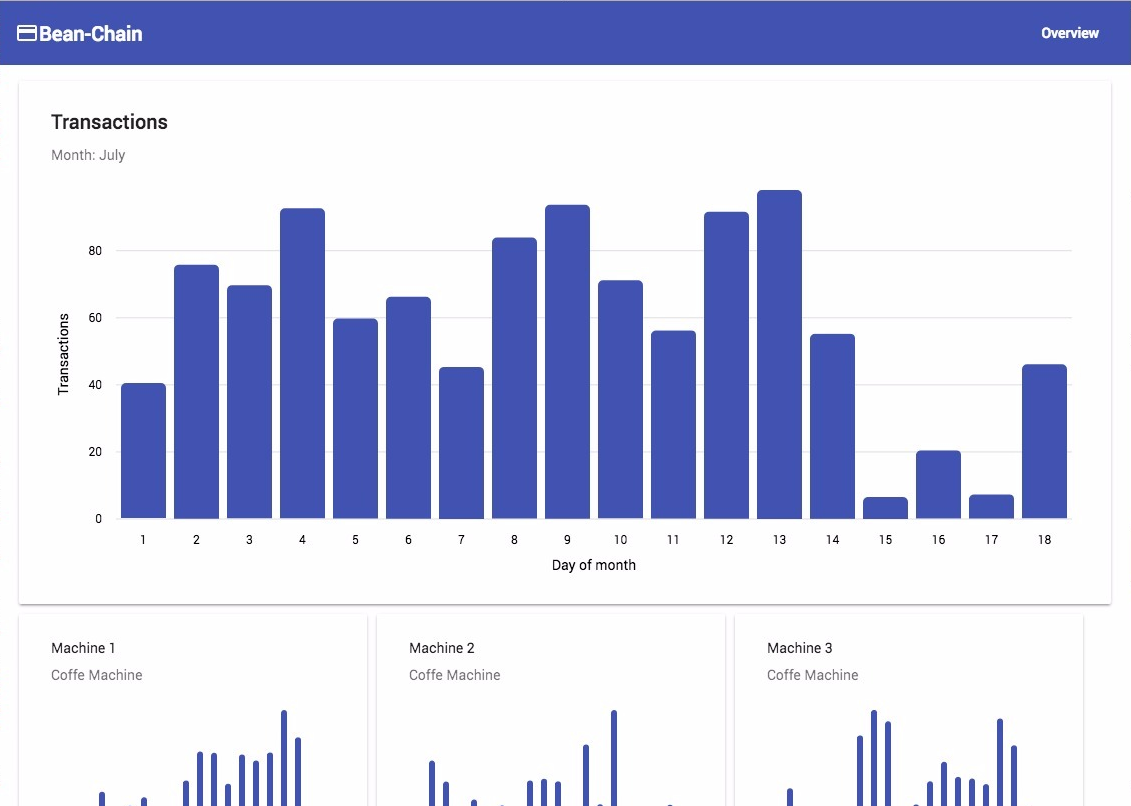
\includegraphics[width=0.49\textwidth]{assets/managment.png}
\caption{Management and analytics of vending machines}
\label{fig:management}
\end{figure}
The management application enables the stakeholders to get an overview of transactions linked to the vending machines manged by each stakeholder. The location owners can see all transactions regarding the vending machines of the locations. The contractors can manage all machines, which they maintain on different locations. The device manufactures have the highest level of visibility and can view  all the machines managed by their contractors. All stakeholder have the ability to make strategic decisions based on analytical insights provided by the management application. For instance, a contractor could decide based on the performance of a location to reallocate vending machines between locations. Further faulty vending machines can be detected by visually analyzing the transactions and identifying missing transactions.

\subsubsection{Payment provider}
The payment provider is the gateway between the distributed ledger of the Hyperledger Fabric framework and the payment provider. Any payment provider, whether decentralized or centralized, can be connected by implementing the application interface to the distributed ledger network. For this purpose, the presented method exposes a REST-API and provides authentication certificates for each payment provider. The implementation of the payment provider depends on the application interface of the provider. For instance an Ethereum based payment provider could leverage smart contracts to notify the distributed ledger on received payments. \\
The payment provider interface can also be used to implement a hardware based payment terminal to accept cash as a source for recharging the balance of a customer.
\section{Experimental results\textsuperscript{2}}
For a proof-of-concept implementation of the proposed architecture, we implemented the management of a coffee vending machine (Figure \ref{fig:coffeemachine}) at the computer science faculty at the Bielefeld University of Applied Sciences (Campus Minden).
\begin{figure}[ht]
    \centering
    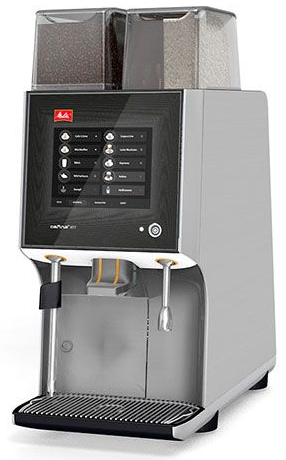
\includegraphics[width=0.3\textwidth]{assets/cafina-xt7.png}
    \caption{Melitta Cafina XT7 coffee machine}
    \label{fig:coffeemachine}
\end{figure}
In this implementation, a Raspberry Pi is physically located next to the coffee machine and is connected to the machines RS232 serial port, which provides the Coffee Credit Interface (CCI) \cite{csi:online} and is intended for external payment devices, like banknote or coin counters.
The Raspberry Pi has internet access and additionally provides a Bluetooth module by which customers can identify themself for payment of various coffee products.
The Raspberry Pi, the customer mobile app and the management application for all stakeholders connect to the cloud-based Hyperledger Fabric instance, were vending machine, settings and account balances are stored. Additionally a fake payment provider is implemented in order to deposit credits without actually making payments.

For evaluation of the proposed architecture, we compare the implemented proof-of-concept with the requirements defined in the Methods section.
Because the proof-of-concept is built using a permissioned blockchain approach, interaction with the entire system is possible without paying transaction fees. With that, the management of vending machines, or in this case the coffee machine, also does not generate costs. The distributed ledger, which is shared between all stakeholders ensures transparency of transaction history and avoids manipulation by any participant of the network.

\begin{figure}[ht]
    \centering
    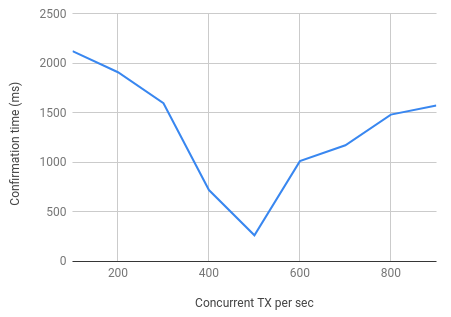
\includegraphics[width=0.5\textwidth]{assets/benchmark.png}
    \caption{Concurrent transactions benchmark}
    \label{fig:benchmark}
\end{figure}
For further evaluation, we benchmarked the transaction throughput of the proposed architecture. Figure \ref{fig:benchmark} shows the lowest confirmation time of around 250 milliseconds at 500 transactions per second, which matches with the configured blocksize of 500 transactions. This value marks the lowest confirmation time, because a new block is instantly filled. Lower and higher transaction-per-second values result in higher confirmation times, which are still acceptable. In these cases the maximum blocktime is triggered at which point a block is finalized. These values fulfill the essential requirement of the system regarding transaction speed and are even lower than EC payment transaction speed.
With the payment provider interface, the system allows the future integration or replacement of payment providers. 
Regarding the user experience requirements, the use of common smartphones, Bluetooth technology and a simple payment application ensures low barriers for interaction with the system for customers. The statistics and configuration capability provided by the management application allows insight into sales figures and enables stakeholder to make strategic decisions about vending machine deployment.

\section{Conclusion\textsuperscript{1}}
In this paper, we proposed an architecture for management and payment processing of vending machines between the triangular business relationship: manufacturer, contractor and location provider. We compared different Distributed Ledger Technologies and implemented a proof-of-concept for a coffee machine. The proof-of-concept implementation showed that the requirements defined in the Section Methods, can indeed be fulfilled with a permissioned blockchain approach. It also revealed difficulties of the customer identification via Bluetooth. In general the detection distance of Beacon is only controlled by the sensitivity of the receiver, while the sender is not able to reduce its transmission power. With this, a nearby attacker is able to receive and clone the Beacon information in order to identify and pay with the victims account. Future improvements of the proposed solution would be, to implement alternatives to Bluetooth Beacons or the usage of onetime Beacons.  

While the proposed approach provides only basic analytical insights, future development could provide advanced sales forecasting capabilities and vending machine fault detection by automated analyzing of the transaction history.

% \clearpage

% BibTeX users please use
\bibliographystyle{template_files/spmpsci.bst}
\bibliography{0_bibliography}   % name your BibTeX data base

% Einige Beispiele die später entfernt werden können
%
\clearpage

\section{Section title}
\label{sec:1}
Citations \cite{8338177} and \cite{8306880} and \cite{8338177}.
\subsection{Subsection title}
\label{sec:2}
as required. Don't forget to give each section
and subsection a unique label (see Sect.~\ref{sec:1}).
\paragraph{Paragraph headings} Use paragraph headings as needed.
\begin{equation}
a^2+b^2=c^2
\end{equation}

\section{Conclusion}
Conclusion is important...

% For one-column wide figures use
\begin{figure}
\centering
% Use the relevant command to insert your figure file.
% For example, with the graphicx package use
  
\includegraphics{template_files/example.eps}
% figure caption is below the figure
\caption{Please write your figure caption here}
\label{fig:1}       % Give a unique label
\end{figure}
%
% For two-column wide figures use
\begin{figure*}
\centering
% Use the relevant command to insert your figure file.
% For example, with the graphicx package use
  
\includegraphics[width=0.75\textwidth]{template_files/example.eps}
% figure caption is below the figure
\caption{Please write your figure caption here}
\label{fig:2}       % Give a unique label
\end{figure*}
%
% For tables use
\begin{table}[t]
% table caption is above the table
\caption{Please write your table caption here}
\centering
\label{tab:1}       % Give a unique label
% For LaTeX tables use
\begin{tabular}{lll}
\hline\noalign{\smallskip}
first & second & third  \\[3pt]
\tableheadseprule\noalign{\smallskip}
number & number & number \\
number & number & number \\
\noalign{\smallskip}\hline
\end{tabular}
\end{table}


\end{document}
% end of file template.tex
